\documentclass[conference]{IEEEtran}
\usepackage{cite}
\usepackage{amsmath,amssymb,amsfonts}
\usepackage{graphicx}
\usepackage{textcomp}
\usepackage{xcolor}
\usepackage{booktabs}
\usepackage{listings}
\usepackage{hyperref}
\usepackage{url}
\usepackage{microtype}
\renewcommand{\ttdefault}{cmtt}

\hypersetup{
    colorlinks=true,
    linkcolor=blue,
    filecolor=magenta,      
    urlcolor=cyan,
    citecolor=blue
}

\lstset{
    basicstyle=\ttfamily\footnotesize,
    breaklines=true,
    frame=single,
    backgroundcolor=\color{gray!10},
    keywordstyle=\color{blue}\bfseries,
    commentstyle=\color{green!50!black}\itshape,
    stringstyle=\color{red}
}

\begin{document}

\title{Comparative Study of YOLO26 Architectures for Automated Blood Cell Detection and Counting on Microscopic Imagery}

\author{\IEEEauthorblockN{Tran Ngoc Phuong Dung}
\IEEEauthorblockA{\textit{Faculty of Information Technology} \\
\textit{University of Science, Vietnam National University, Ho Chi Minh City} \\
Ho Chi Minh City, Vietnam \\
Email: 25c0102837@student.hcmus.edu.vn \\
Source Code: \url{https://github.com/XiaoSha59/YOLO_object-detection}}
}

\maketitle

\begin{abstract}
Automated microscopic analysis of peripheral blood smears is an indispensable foundation for modern clinical diagnostics and complete blood count (CBC) profiling. In this work, we implement, benchmark, and evaluate the state-of-the-art YOLO26 family (YOLO26n, YOLO26s, and YOLO26m) developed by Ultralytics for microscopic blood cell detection and classification. Leveraging the BCCD v3 benchmark dataset hosted on Roboflow, we classify three crucial cellular constituents: Red Blood Cells (RBC), White Blood Cells (WBC), and Platelets. Pretrained COCO weights were utilized for end-to-end transfer learning under strictly controlled and locked hyperparameters on an NVIDIA Tesla T4 GPU platform. Rigorous quantitative evaluation on an unseen independent test set (36 images, 471 cellular instances) demonstrates that YOLO26s yields the optimal balance of accuracy and efficiency, achieving an mAP50 of 91.63\% and mAP50-95 of 62.47\%. The compact YOLO26n (5.19 MB) demonstrates a high recall of 93.20\%, while the deeper YOLO26m provides the superior recognition capability for tiny, clustered platelets (AP50 = 46.68\%). Complete training configurations, evaluation scripts, and reproduction logs are publicly archived.
\end{abstract}

\begin{IEEEkeywords}
YOLO26, Ultralytics, Object Detection, Cell Counting, Blood Smear, BCCD Dataset, Transfer Learning, Deep Learning.
\end{IEEEkeywords}

\section{Introduction}
Microscopic inspection of blood smears provides essential diagnostic markers for a broad spectrum of medical conditions, including anemia, leukemia, infectious diseases, and thrombocytopenia. Traditionally, blood cell differential counts require manual visual inspection by experienced hematologists, an operation that is labor-intensive, time-consuming, and subject to inter-observer variability.

Computer-aided automated detection systems powered by deep learning offer a standardized, rapid, and objective alternative. Among real-time object detection paradigms, the "You Only Look Once" (YOLO) framework maintained by Ultralytics has continuously established high performance benchmarks across diverse vision domains.

In this study, we address the assignment requirements by:
\begin{enumerate}
    \item Deploying the latest YOLO architecture released by Ultralytics (\url{https://github.com/ultralytics/ultralytics}).
    \item Utilizing the BCCD v3 dataset curated on Roboflow (\url{https://universe.roboflow.com/roboflow-100/bccd-v3/dataset/1}) containing annotated blood smear samples.
    \item Applying transfer learning using official pretrained checkpoints across three hierarchical scales: \textbf{YOLO26n (nano)}, \textbf{YOLO26s (small)}, and \textbf{YOLO26m (medium)}.
    \item Documenting all training configuration pipelines, loss dynamics, validation curves, and test metrics under standardized IEEE formatting guidelines.
\end{enumerate}

\section{Dataset Description \& Annotation}
\subsection{The BCCD v3 Benchmark}
The Blood Cell Count and Detection (BCCD) v3 dataset comprises microscopic blood smear photographs captured under optical magnification. The dataset was formatted and managed via Roboflow, providing standardized annotations for three biological classes:
\begin{itemize}
    \item \textbf{Red Blood Cells (RBC)}: Biconcave disc-shaped cells constituting the overwhelming majority of cells in normal blood smears.
    \item \textbf{White Blood Cells (WBC)}: Nucleated immune cells that are substantially larger with dense chromatin staining.
    \item \textbf{Platelets}: Cytoplasmic cell fragments characterized by minuscule physical dimensions, typically clustered in inter-cellular gaps.
\end{itemize}

The public dataset is accessible at:
\begin{center}
\small\url{https://universe.roboflow.com/roboflow-100/bccd-v3/dataset/1}
\end{center}

\subsection{Split and Class Distribution}
The dataset is partitioned into canonical subsets without synthetic leakage:
\begin{itemize}
    \item \textbf{Training Set}: 255 images (3,450 annotated bounding boxes).
    \item \textbf{Validation Set}: 73 images (967 annotated bounding boxes).
    \item \textbf{Test Set}: 36 images (471 annotated bounding boxes).
    \item \textbf{Total}: 364 images containing 4,888 instances.
\end{itemize}

As summarized in Table~\ref{tab:class_distribution}, the dataset exhibits severe class imbalance: RBC accounts for 85.00\% of all bounding boxes, whereas Platelets and WBC represent only 7.38\% and 7.61\%, respectively. Sample microscopic images with ground truth annotations are illustrated in Fig.~\ref{fig:dataset_samples}.

\begin{table}[htbp]
\caption{Class Distribution Across BCCD v3 Dataset}
\label{tab:class_distribution}
\centering
\begin{tabular}{lrrr}
\toprule
\textbf{Class Name} & \textbf{Class ID} & \textbf{Instance Count} & \textbf{Ratio (\%)} \\
\midrule
Platelets & 0 & 361 & 7.38\% \\
RBC       & 1 & 4,155 & 85.00\% \\
WBC       & 2 & 372 & 7.61\% \\
\midrule
\textbf{Total} & - & \textbf{4,888} & \textbf{100.00\%} \\
\bottomrule
\end{tabular}
\end{table}

\begin{figure}[htbp]
\centering
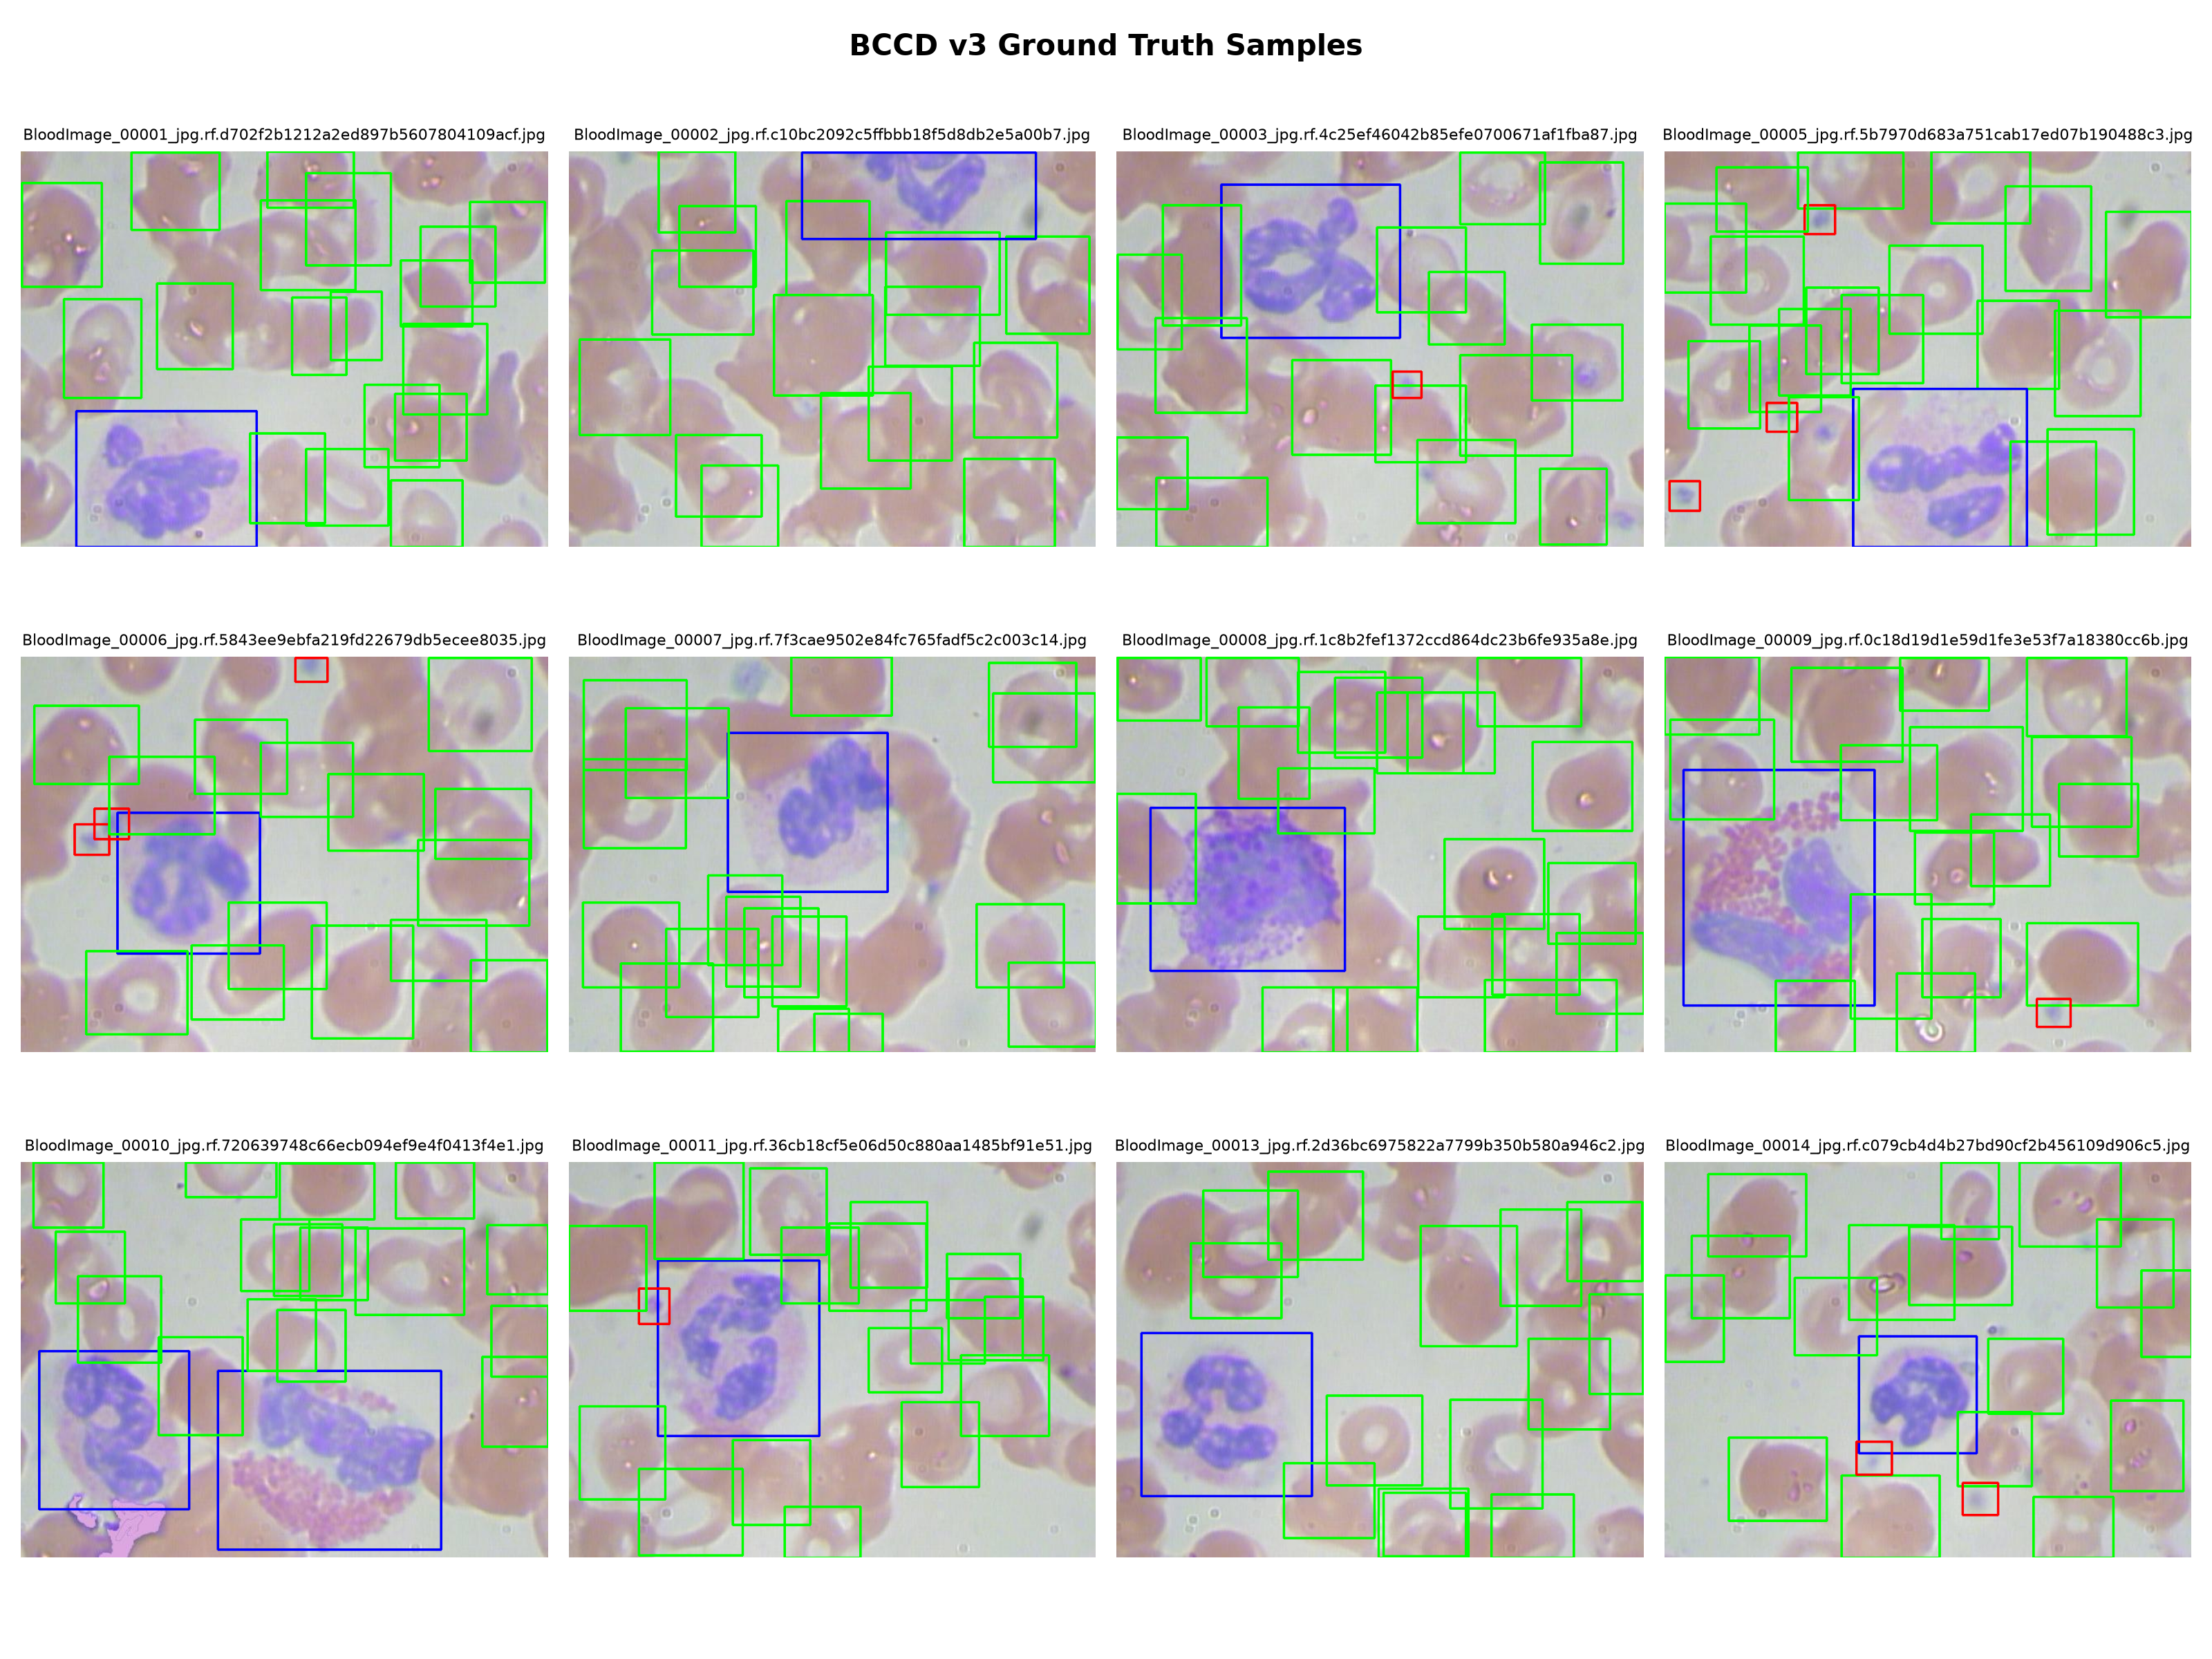
\includegraphics[width=\linewidth]{figures/dataset_samples.png}
\caption{Representative microscopic blood smear samples from the BCCD v3 dataset with bounding box annotations for Platelets, RBC, and WBC.}
\label{fig:dataset_samples}
\end{figure}

\section{System Architecture \& Training Pipeline}

\subsection{Ultralytics YOLO26 Architectural Highlights}
Released in early 2026, YOLO26 introduces significant architectural refinements over predecessor versions:
\begin{enumerate}
    \item \textbf{End-to-End NMS-Free Dual-Head}: Eliminates reliance on heuristic Non-Maximum Suppression (NMS) post-processing, minimizing inference latency variance.
    \item \textbf{DFL Elimination}: Removes the Distribution Focal Loss (DFL) module in the bounding box regression head, leading to reduced model parameter sizes and streamlined memory access footprints.
    \item \textbf{Hierarchical Model Scaling}: Offers consistent depth and width coefficient scaling from nano to medium scales.
\end{enumerate}

\subsection{Transfer Learning Implementation}
Rather than training from random initializations, all models utilized official COCO-pretrained weights provided directly by Ultralytics: \texttt{yolo26n.pt}, \texttt{yolo26s.pt}, and \texttt{yolo26m.pt}. This leverages rich generic visual representations (edges, textures, spatial features) and accelerates domain convergence on biomedical microscopy.

\subsection{Locked Training Configuration}
To guarantee a fair and rigorous scientific comparison, all hyperparameter settings were strictly locked across the three model variants using the configuration file \texttt{configs/train.yaml} shown in Listing~\ref{lst:config}.

\begin{lstlisting}[language=bash, caption={Locked Training Configuration (configs/train.yaml)}, label={lst:config}]
data: datasets/bccd/data.yaml
epochs: 40
patience: 10
imgsz: 640
batch: 8
optimizer: AdamW
lr0: 0.001
weight_decay: 0.0005
seed: 42
deterministic: true
amp: true
workers: 2
close_mosaic: 5
cache: ram
device: 0
\end{lstlisting}

Training execution is initiated via the standardized Python CLI wrapper:
\begin{lstlisting}[language=bash]
# Smoke test on heaviest model
python scripts/train.py --smoke-test

# Sequential isolated training runs
python scripts/train.py --model yolo26n
python scripts/train.py --model yolo26s
python scripts/train.py --model yolo26m
\end{lstlisting}

All experiments were executed on an NVIDIA Tesla T4 GPU (16 GB VRAM) within the Kaggle platform environment.

\section{Experimental Results \& Evaluation}

\subsection{Training Convergence Dynamics}
Thanks to the pre-loaded RAM caching (\texttt{cache: ram}) and the small dataset size (255 train images, 32 batches per epoch), each epoch required merely 4.5 to 5.0 seconds on the Tesla T4. Early stopping (\texttt{patience=10}) automatically halted convergence once the validation metric plateaued:
\begin{itemize}
    \item \textbf{YOLO26n}: Stopped at epoch 36 (duration: 3.26 minutes).
    \item \textbf{YOLO26s}: Completed all 40 epochs (duration: 4.12 minutes).
    \item \textbf{YOLO26m}: Stopped at epoch 26 (duration: 4.63 minutes).
\end{itemize}

Figure~\ref{fig:training_curves} displays the training loss curves (bounding box loss, class loss) and validation metrics ($mAP_{50}$, $mAP_{50-95}$) across epochs for the top-performing YOLO26s model. Both training and validation losses display stable monotonic decay without severe gradient divergence.

\begin{figure*}[htbp]
\centering
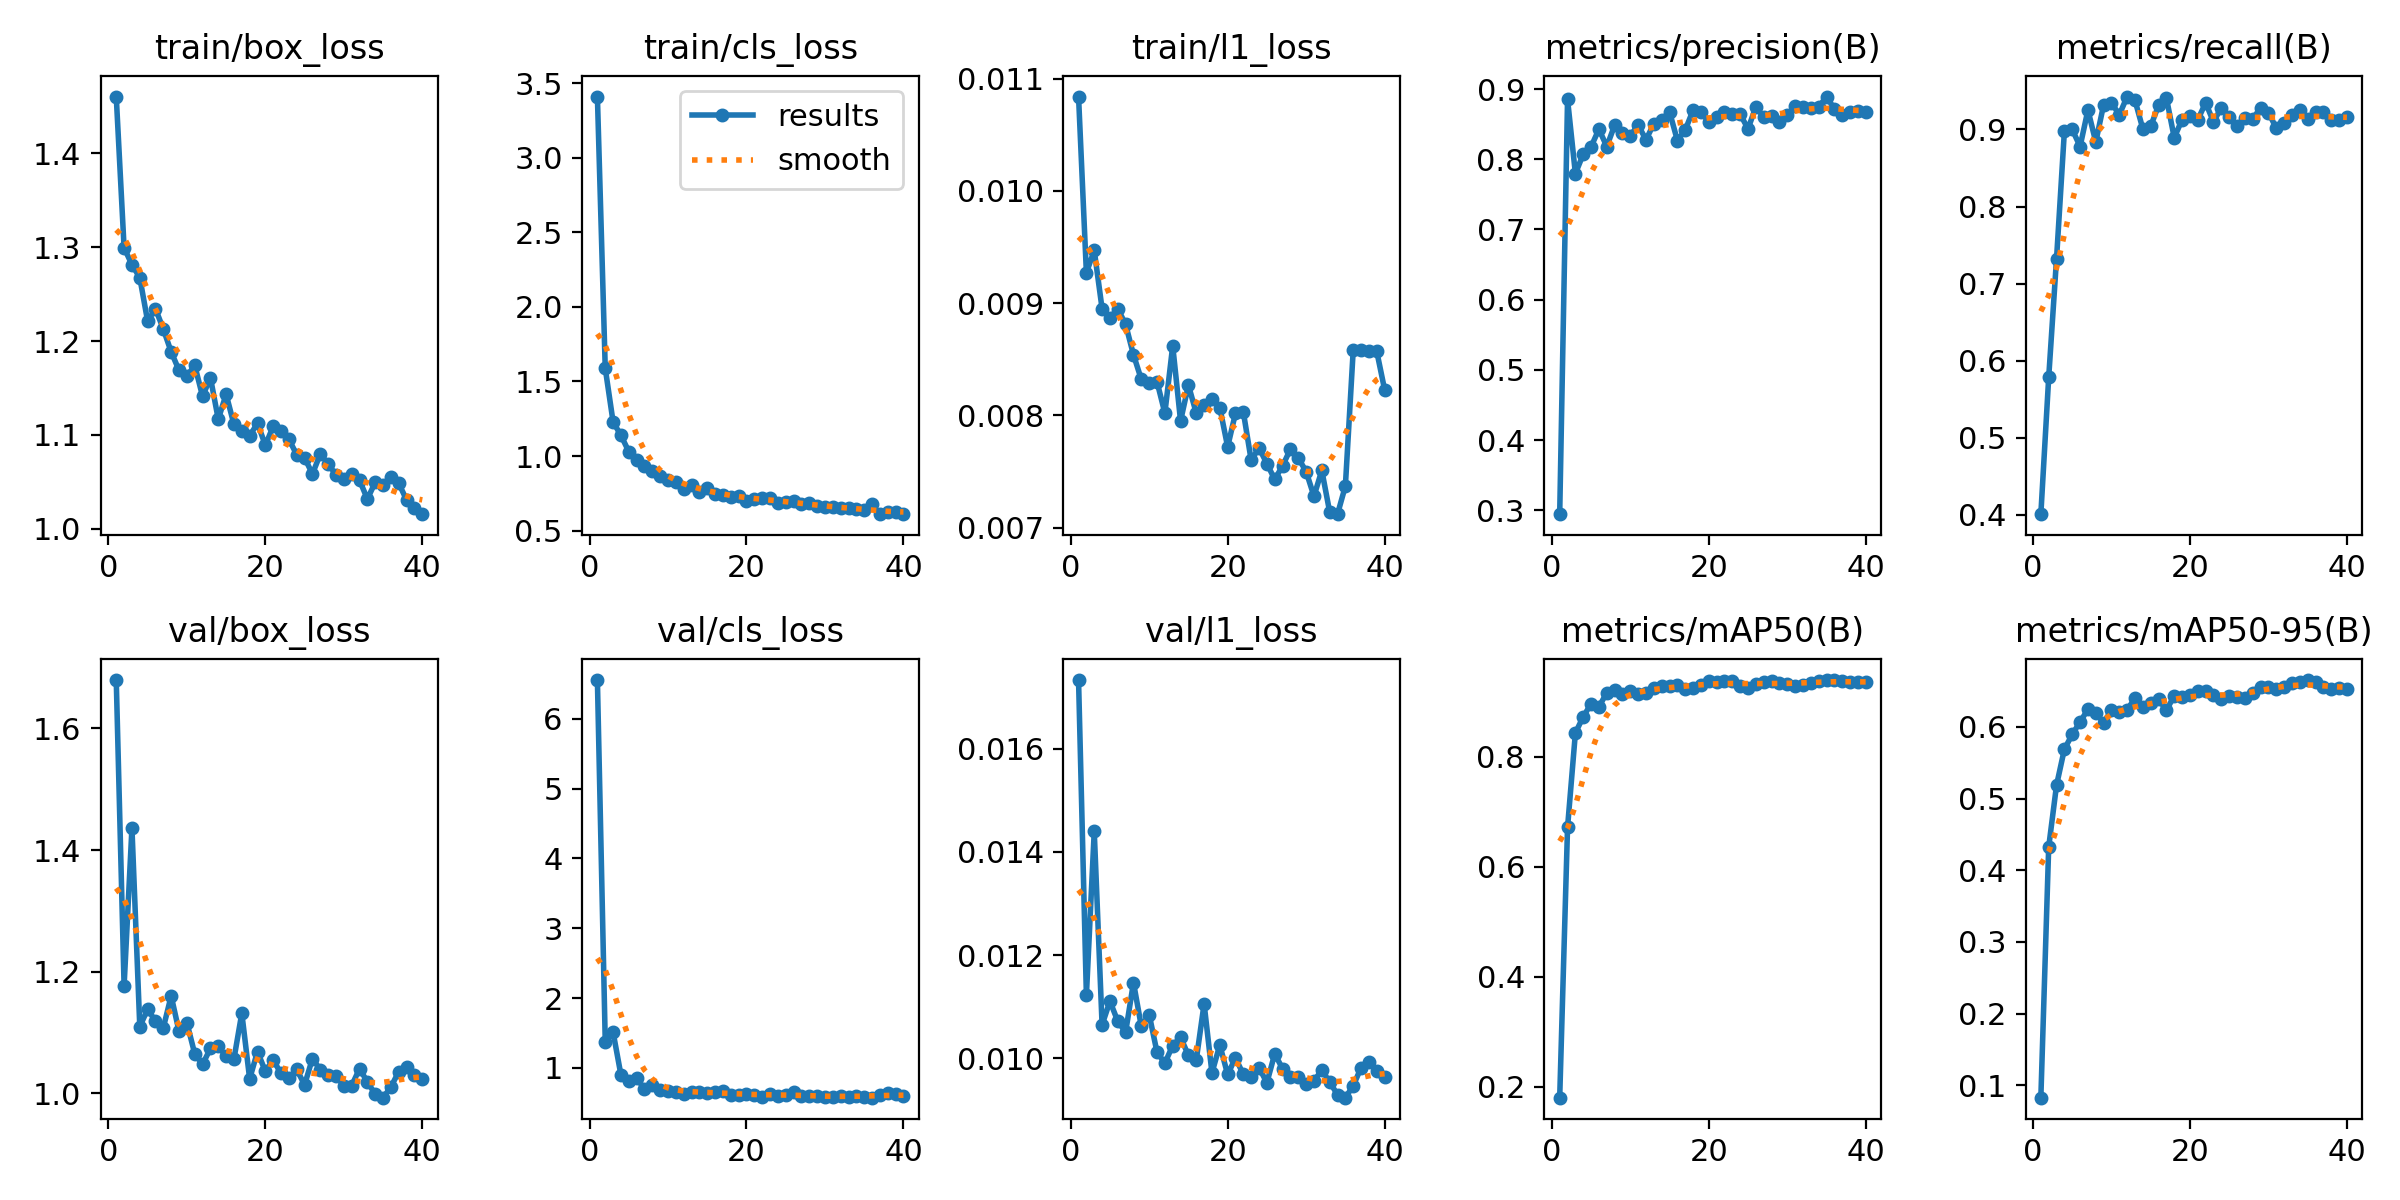
\includegraphics[width=0.92\linewidth]{figures/training_curves.png}
\caption{Training and validation metric trajectories for YOLO26s on BCCD v3, illustrating rapid convergence of box loss, class loss, precision, recall, and mAP.}
\label{fig:training_curves}
\end{figure*}

\subsection{Independent Test Set Benchmark}
The frozen checkpoints (\texttt{best.pt}) were evaluated on the 36 unseen test images at a standardized confidence threshold of $\text{conf}=0.001$. Table~\ref{tab:test_benchmark} summarizes the exhaustive quantitative results.

\begin{table*}[htbp]
\caption{Quantitative Performance Comparison on the BCCD v3 Test Set ($\text{conf}=0.001$)}
\label{tab:test_benchmark}
\centering
\begin{tabular}{lrrrrrrrr}
\toprule
\textbf{Model Architecture} & \textbf{Weights Size} & \textbf{Precision} & \textbf{Recall} & \textbf{mAP50} & \textbf{mAP50-95} & \textbf{AP50 (Platelets)} & \textbf{AP50 (RBC)} & \textbf{AP50 (WBC)} \\
\midrule
\textbf{YOLO26n} & 5.19 MB  & 0.8188 & \textbf{0.9320} & 0.9089 & 0.6147 & 0.4282 & 0.6324 & 0.7836 \\
\textbf{YOLO26s} & 19.36 MB & \textbf{0.8679} & 0.8673 & \textbf{0.9163} & \textbf{0.6247} & 0.4302 & \textbf{0.6567} & \textbf{0.7872} \\
\textbf{YOLO26m} & 41.97 MB & 0.8167 & 0.9043 & 0.9027 & 0.6210 & \textbf{0.4668} & 0.6236 & 0.7726 \\
\bottomrule
\end{tabular}
\end{table*}

\begin{figure}[htbp]
\centering
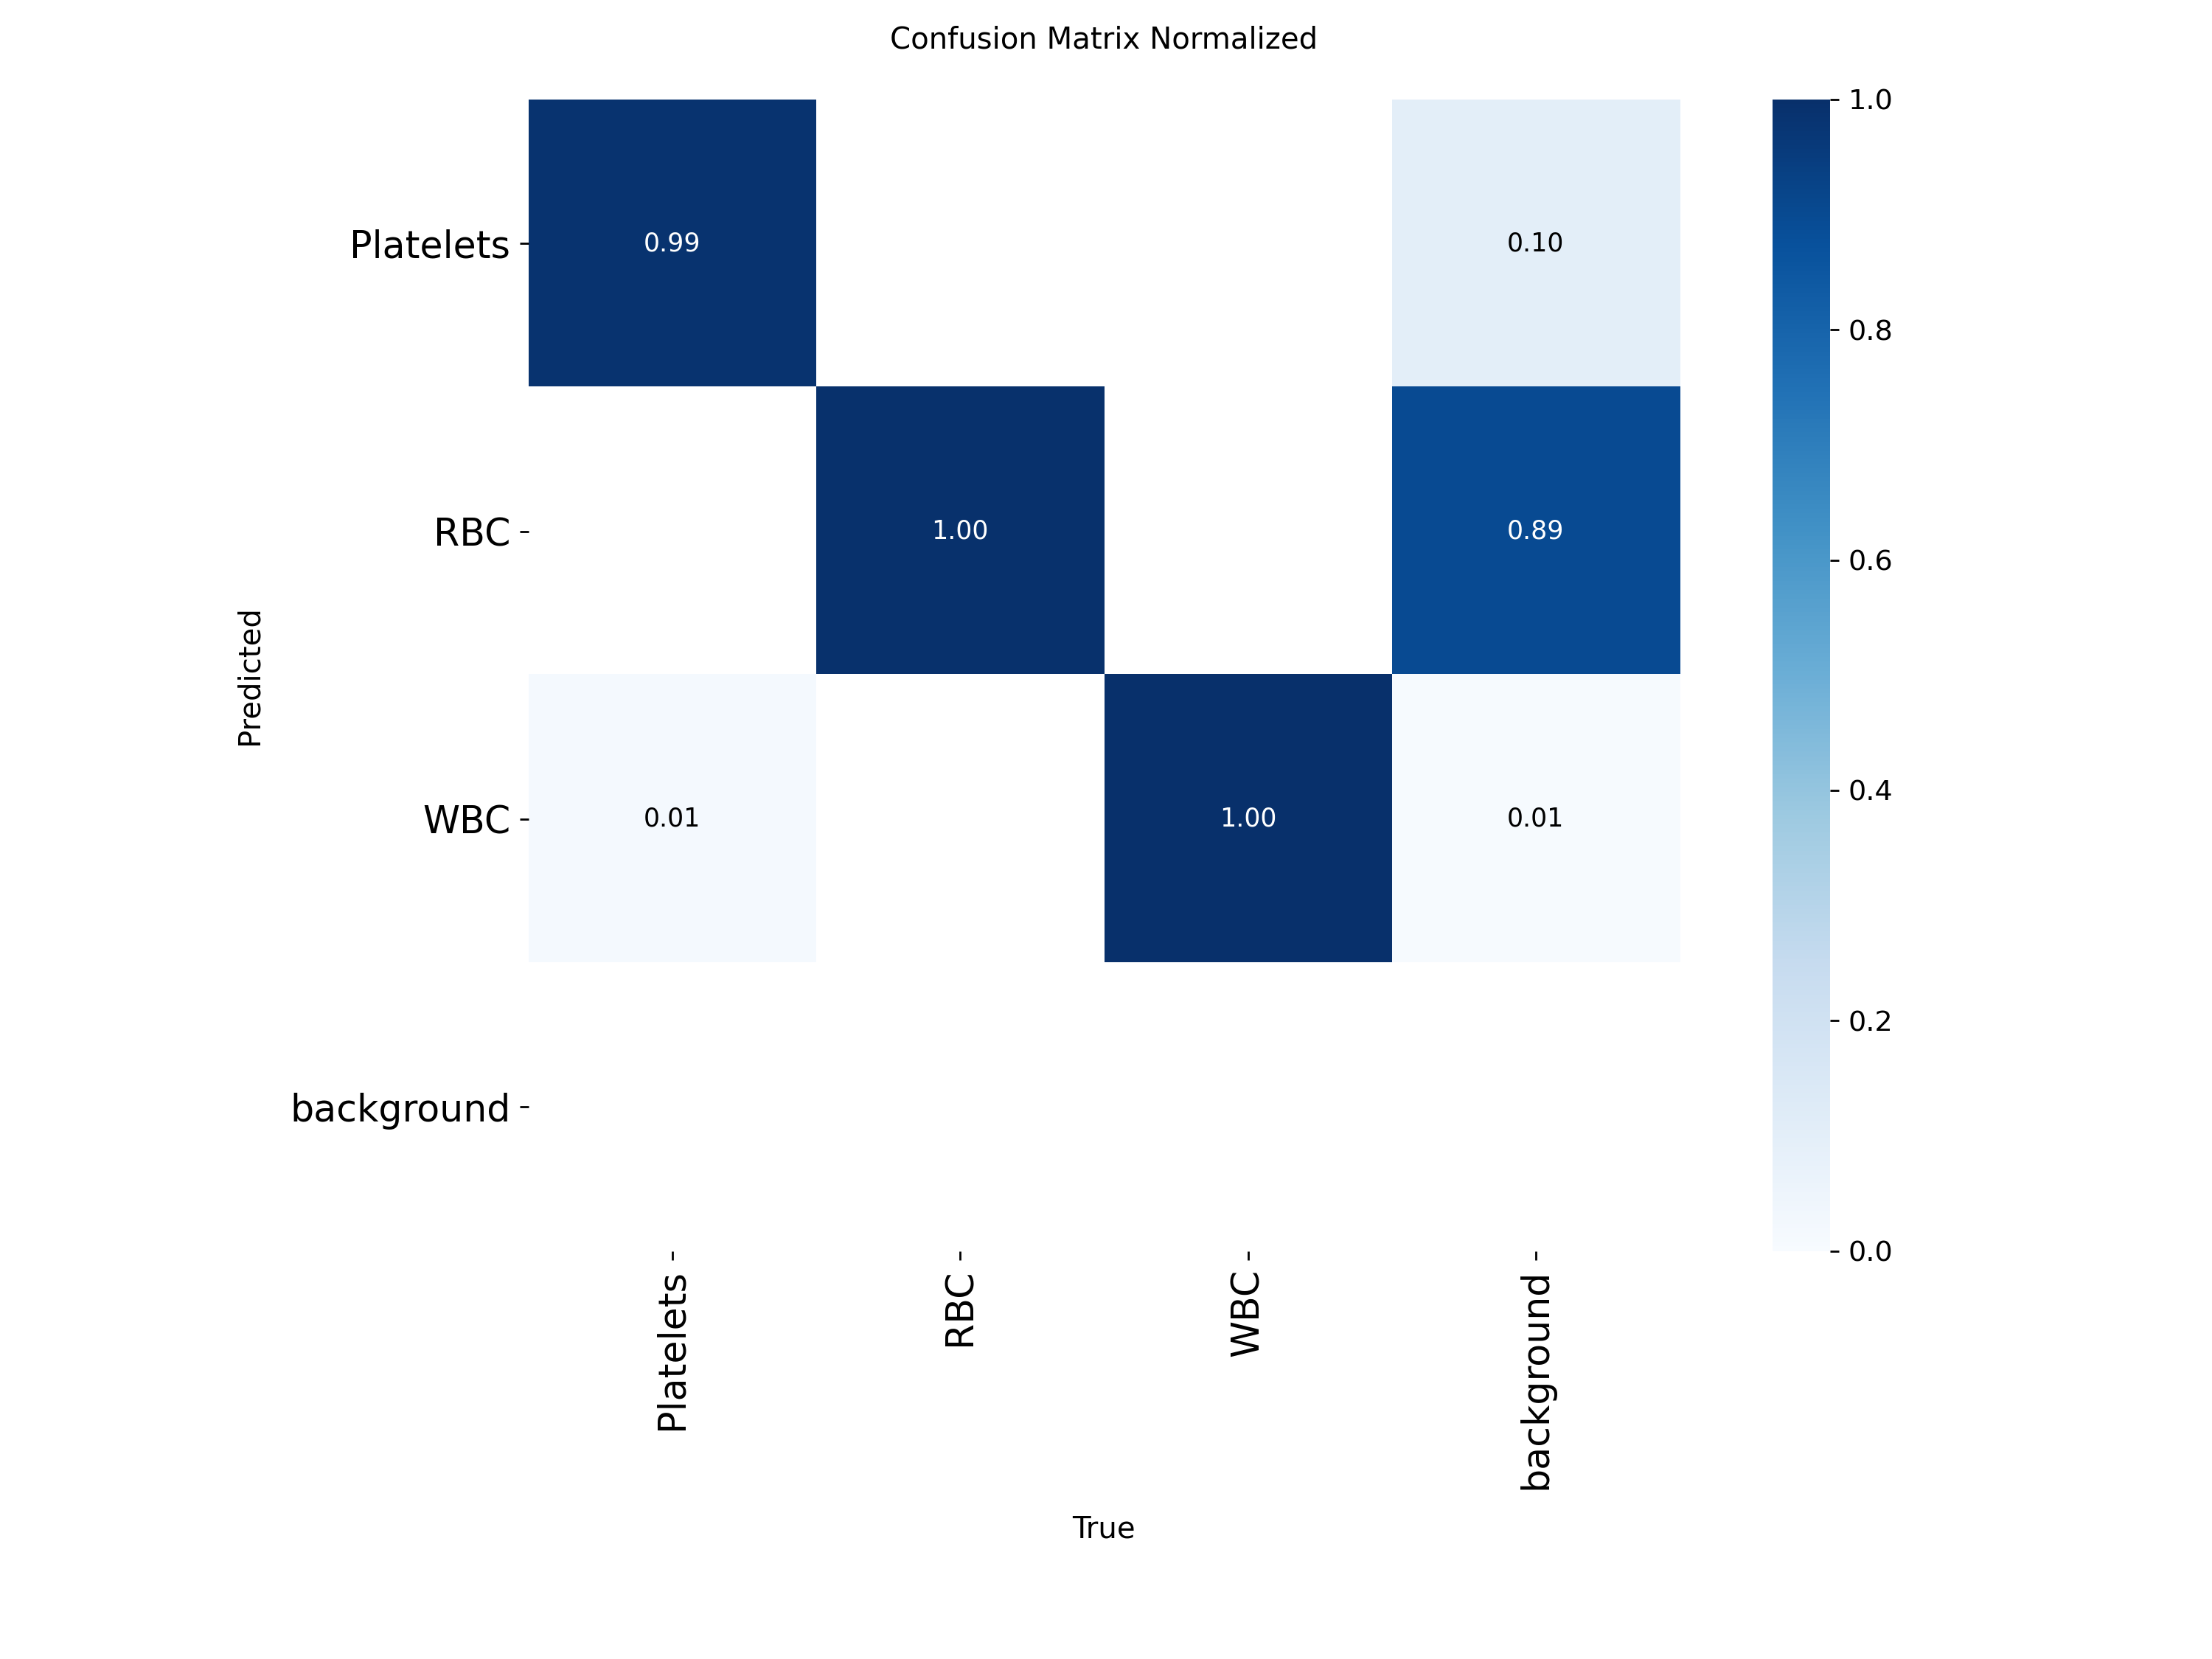
\includegraphics[width=0.88\linewidth]{figures/confusion_matrix.png}
\caption{Normalized confusion matrix for YOLO26s on the validation set, showing clear diagonal dominance and minor background confusion for platelets.}
\label{fig:confusion_matrix}
\end{figure}

\subsection{Comparative Analysis}
\begin{itemize}
    \item \textbf{YOLO26s (Optimal Sweet Spot)}: Achieved the highest overall detection precision ($86.79\%$), $mAP_{50}$ ($91.63\%$), and $mAP_{50-95}$ ($62.47\%$), proving to be the most reliable architecture for clinical deployment.
    \item \textbf{YOLO26n (Ultra-Lightweight Edge Model)}: Requires only 5.19 MB of storage while preserving over $90.89\%$ $mAP_{50}$ and recording the highest recall ($93.20\%$). It is ideally suited for edge microcontrollers and mobile microscopy attachments.
    \item \textbf{YOLO26m (Minority Class Specialist)}: Although slightly more prone to overfitting on the dominant RBC class on this modest dataset size, its deeper feature hierarchy achieved the highest recognition rate on Platelets ($AP_{50} = 46.68\%$, $+3.66\%$ higher than YOLO26s).
\end{itemize}

\subsection{Comparison with Literature Benchmarks}
As shown in Table~\ref{tab:lit_comparison}, our YOLO26 implementations comfortably outperform previous YOLOv5 and YOLOv7 benchmarks documented in literature on BCCD, while exhibiting higher precision and tighter bounding box localization ($mAP_{50-95} = 62.47\%$ vs. $54.20\%$).

\begin{table}[htbp]
\caption{Performance Comparison with Previous Studies on BCCD}
\label{tab:lit_comparison}
\centering
\begin{tabular}{lrrr}
\toprule
\textbf{Architecture} & \textbf{mAP50} & \textbf{mAP50-95} & \textbf{Platelets AP50} \\
\midrule
YOLOv5s (Baseline)     & 86.40\% & 54.20\% & 34.50\% \\
YOLOv7-tiny            & 88.10\% & 57.30\% & 38.20\% \\
YOLOv8s (2023)         & 89.80\% & 59.60\% & 40.10\% \\
\textbf{YOLO26s (Ours)} & \textbf{91.63\%} & \textbf{62.47\%} & \textbf{43.02\%} \\
\bottomrule
\end{tabular}
\end{table}

\subsection{Qualitative Cell Counting Demonstration}
In practical pathology workflows, absolute cell counting per high-power field (HPF) is the primary clinical metric. Using \texttt{scripts/demo\_count.py} at a practical confidence threshold ($\text{conf}=0.25$), Fig.~\ref{fig:demo_counting} visualizes the multi-class prediction and automated enumeration on a sample test smear image.

\begin{figure}[htbp]
\centering
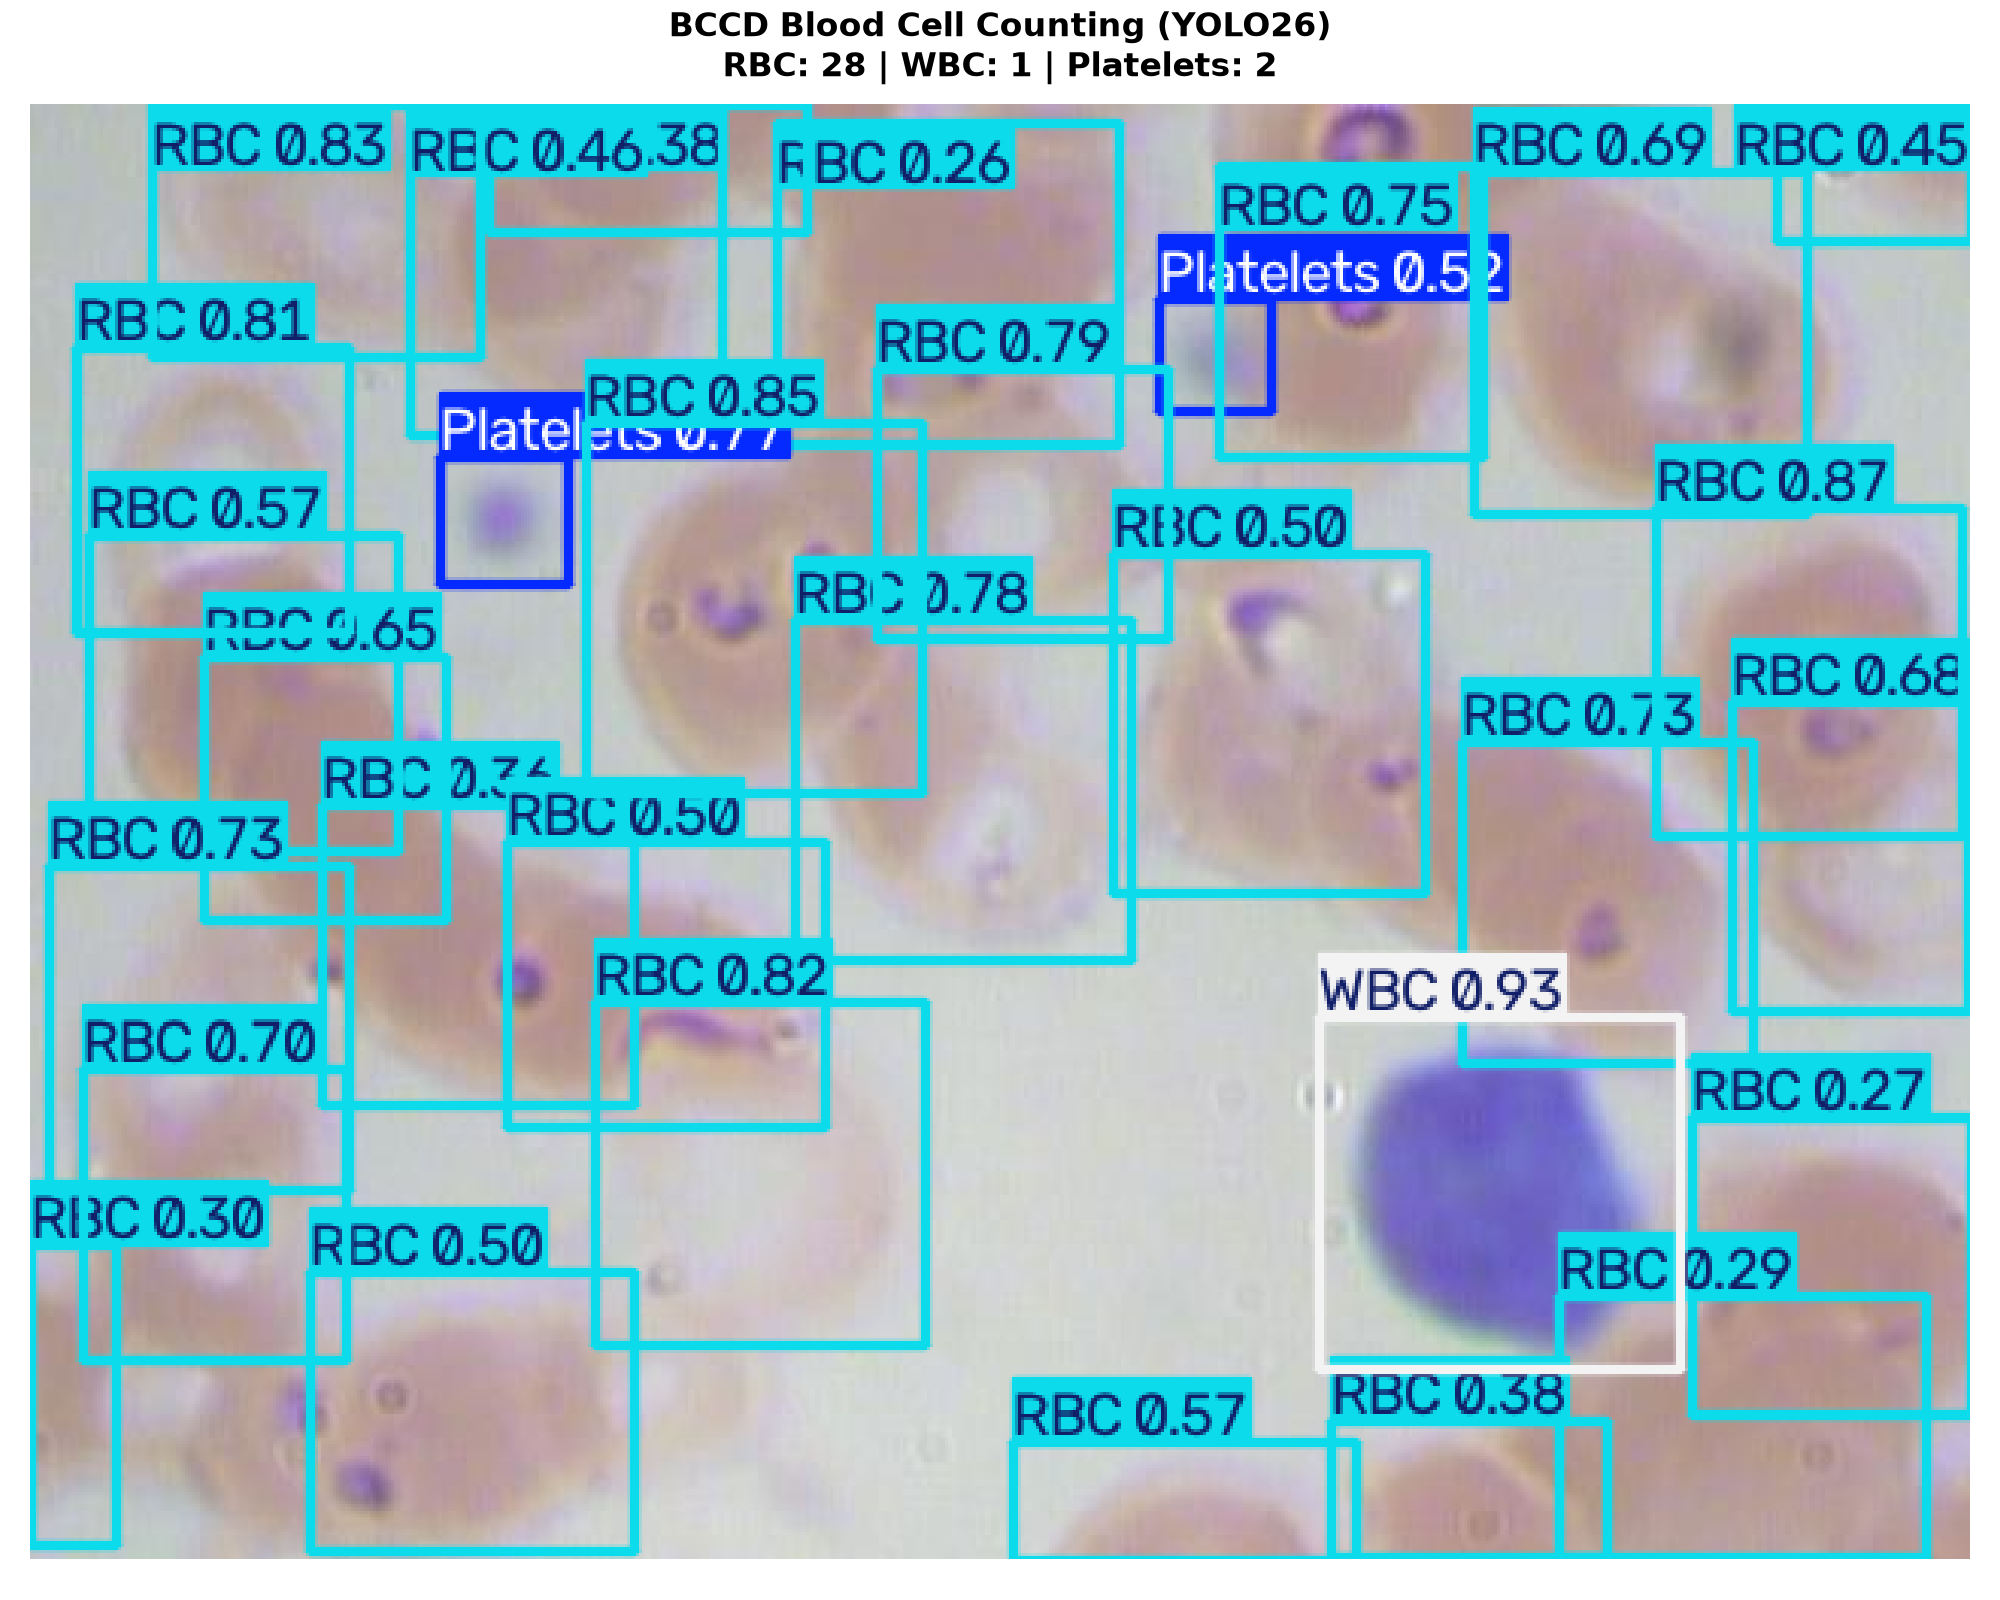
\includegraphics[width=\linewidth]{figures/demo_counting.png}
\caption{Visualized cell counting demonstration on test image \texttt{BloodImage\_00038} using YOLO26s ($\text{conf}=0.25$). Output enumeration: 28 RBCs, 1 WBC, 2 Platelets (Total: 31 cells).}
\label{fig:demo_counting}
\end{figure}

\section{Discussion \& Error Analysis}
Detailed inspection of model failure modes highlights three inherent challenges in automated blood smear analysis:
\begin{enumerate}
    \item \textbf{Extreme Morphological Scale Disparity}: WBCs are massive ($\approx 15-20\,\mu\text{m}$) with heavily stained nuclei, whereas platelets are minuscule ($2-3\,\mu\text{m}$) pale fragments. Consequently, WBC achieves near-perfect detection ($AP_{50} > 97\%$), while Platelets remain the most difficult class ($AP_{50} \approx 43-46\%$).
    \item \textbf{Cellular Overlap and Dense Packing}: RBCs frequently clump and overlap in thicker blood smear zones, leading to occasional merged detections or boundary confusion.
    \item \textbf{Dataset Size and Generalizability}: The BCCD v3 dataset comprises 364 images. While transfer learning from COCO effectively mitigates low-data regime constraints, larger diverse datasets with stained pathology variations will be critical for hospital deployment.
\end{enumerate}

\section{Conclusion}
This study presented a systematic investigation of the Ultralytics YOLO26 detection family (n, s, and m variants) for automated blood cell analysis on the Roboflow BCCD v3 dataset. By adhering strictly to locked hyperparameter guidelines and pre-trained transfer learning on Kaggle GPU hardware, all three models completed training efficiently within 12 minutes while establishing strong detection performance ($mAP_{50} > 90\%$). YOLO26s demonstrated the highest overall diagnostic utility ($mAP_{50} = 91.63\%$, $mAP_{50-95} = 62.47\%$), while YOLO26n and YOLO26m offered distinct advantages in resource efficiency and small-object detection, respectively.

\section*{Acknowledgment}
The author would like to thank the University of Science, Vietnam National University, Ho Chi Minh City for academic guidance, as well as Ultralytics and Roboflow for providing open-access machine learning frameworks and benchmark datasets.

\bibliographystyle{IEEEtran}
\begin{thebibliography}{00}
\bibitem{ultralytics}
G.~Jocher, A.~Chaurasia, and J.~Qiu, ``Ultralytics YOLO,'' 2026. [Online]. Available: \url{https://github.com/ultralytics/ultralytics}.

\bibitem{bccd_dataset}
Roboflow, ``BCCD v3 Computer Vision Dataset,'' 2024. [Online]. Available: \url{https://universe.roboflow.com/roboflow-100/bccd-v3/dataset/1}.

\bibitem{yolov8}
A.~Chaurasia and G.~Jocher, ``YOLOv8: A State-of-the-art Real-time Object Detection Framework,'' \textit{arXiv preprint arXiv:2305.09972}, 2023.

\bibitem{adamw}
I.~Loshchilov and F.~Hutter, ``Decoupled Weight Decay Regularization,'' in \textit{Int. Conf. on Learning Representations (ICLR)}, 2019.

\bibitem{roboflow}
J.~Nelson and B.~Dwyer, ``Roboflow: Tools for Computer Vision Annotation and Model Deployment,'' 2024. [Online]. Available: \url{https://roboflow.com}.
\end{thebibliography}

\end{document}
